%------------------------------%
%% ✎ Dylan (V1) %%%%%%%%% ✅ %%
%% ✎ Alain (V2) %%%%%%%%% ✅ %%
%% ✎ Dylan (V3) %%%%%%%%% ✅ %%
%------------------------------%

\cleardoublepage
\section*{\textsl{Captatio benevolentiae}
    \label{body:mt180}
    }
    \addcontentsline{toc}{part}{\textsl{Captatio benevolentiae}}
    \markboth{\textsl{Captatio benevolentiae}}{}
    \markright{Preface}{}

%\poemtitle{Before Automobility, the Quest for Intermodality}
\subsection*{Before Automobility, the Quest for Intermodality (\textsl{Devant l'Automobilité, la quête de l'Intermodalité}}
    
\settowidth{\versewidth}{And objects at rest tended to remain at rest}
\begin{verse}[\versewidth]

Il était une fois,\\
Au cœur du lointain eldorado lillois,\\
Une splendide Princesse appelée \textsl{Pieds}\\
Épousa le Prince \textsl{Train}, en un lien sacré et privilégié.\\
Cette union vénérée régnait sur la nation,\\
Organisée par des zones piétonnes et des stations.

Or, brusquement, cette relation idyllique\\
Fut renversée par une rivale maléfique.\\
La sorcière \textsl{La Voiture} insuffla un sortilège,\\
Envoûtant ces terres de mille pièges.\\
Le pays se pervertit en périphéries éparpillées.\\
Aux paysages pollués et aux chemins embouteillés.

Afin de briser l’envoûtement de \textsl{La Voiture},\\
Le pouvoir valorisa les gares sans véritable rupture.\\
En vain, les individus véhiculés vivant loin.

Pris de panique, \textsl{Pieds} et \textsl{Train} appelèrent leurs adjoints,\\
Les fidèles \textsl{Bus}, \textsl{Tramway} et \textsl{Métropolitain},\\
Hélas, peu adaptés à l’espace dépeint, rendant l'effort vain.

Las de ces lieux esclaves des lois de l’automobile,\\
Les nobles se tournèrent vers \textsl{Vélo}, un chevalier habile.\\
Surnommé \textsl{La Petite Reine} après son arrivée,\\
\textsl{Vélo} a pour vertu d'étendre les périmètres des gares fortifiées.

Mais, l’énergie conquérante de \textsl{Vélo} étant limitée,\\
Le destrier fut rafistolé par la fée \textsl{Électricité}.\\
Et naquirent dans cette région fantastique\dots\\
Des vélos et trottinettes électriques.\\
Connus sous le nom de \textsl{Mobilité Individuelle Légère},\\
Ces engins variés ont un rôle salutaire,\\
Permettant une combinaison aisée par la population,\\
Améliorant l’accessibilité des stations.

\textsl{Train} et \textsl{Mobilité Individuelle Légère} conclurent une alliance,\\
Une union symbolisée par la correspondance.\\
La Maison \textsl{Intermodalité},\\
Dont la devise est la compétitivité,\\
S'engageait à combiner ces modes conjointement,\\
Au cours du même déplacement.

[\dots]

La province des Hauts-de-France parvint à maîtriser la menace,\\
D’un urbanisme néfaste, sans grâce et inefficace.

D’ailleurs, j’ai un secret, je vous le confie\dots\\
Tou·te·s nos protagonistes dédièrent ce paradis retrouvé,\\
À leur enfant, agréable et cyclable,\\
Qu’ils appelèrent \textsl{Région Durable}.\\
Incroyable~?\\

\end{verse}
\textsl{Finale régionale Ma Thèse en 180 Secondes} (\textcolor{blue}{Dylan Moinse, 2022})

    % Figure MT180
    \begin{figure}[h!]\vspace*{4pt}
        \caption*{}
        \label{fig-preambule:mt180}
        \centerline{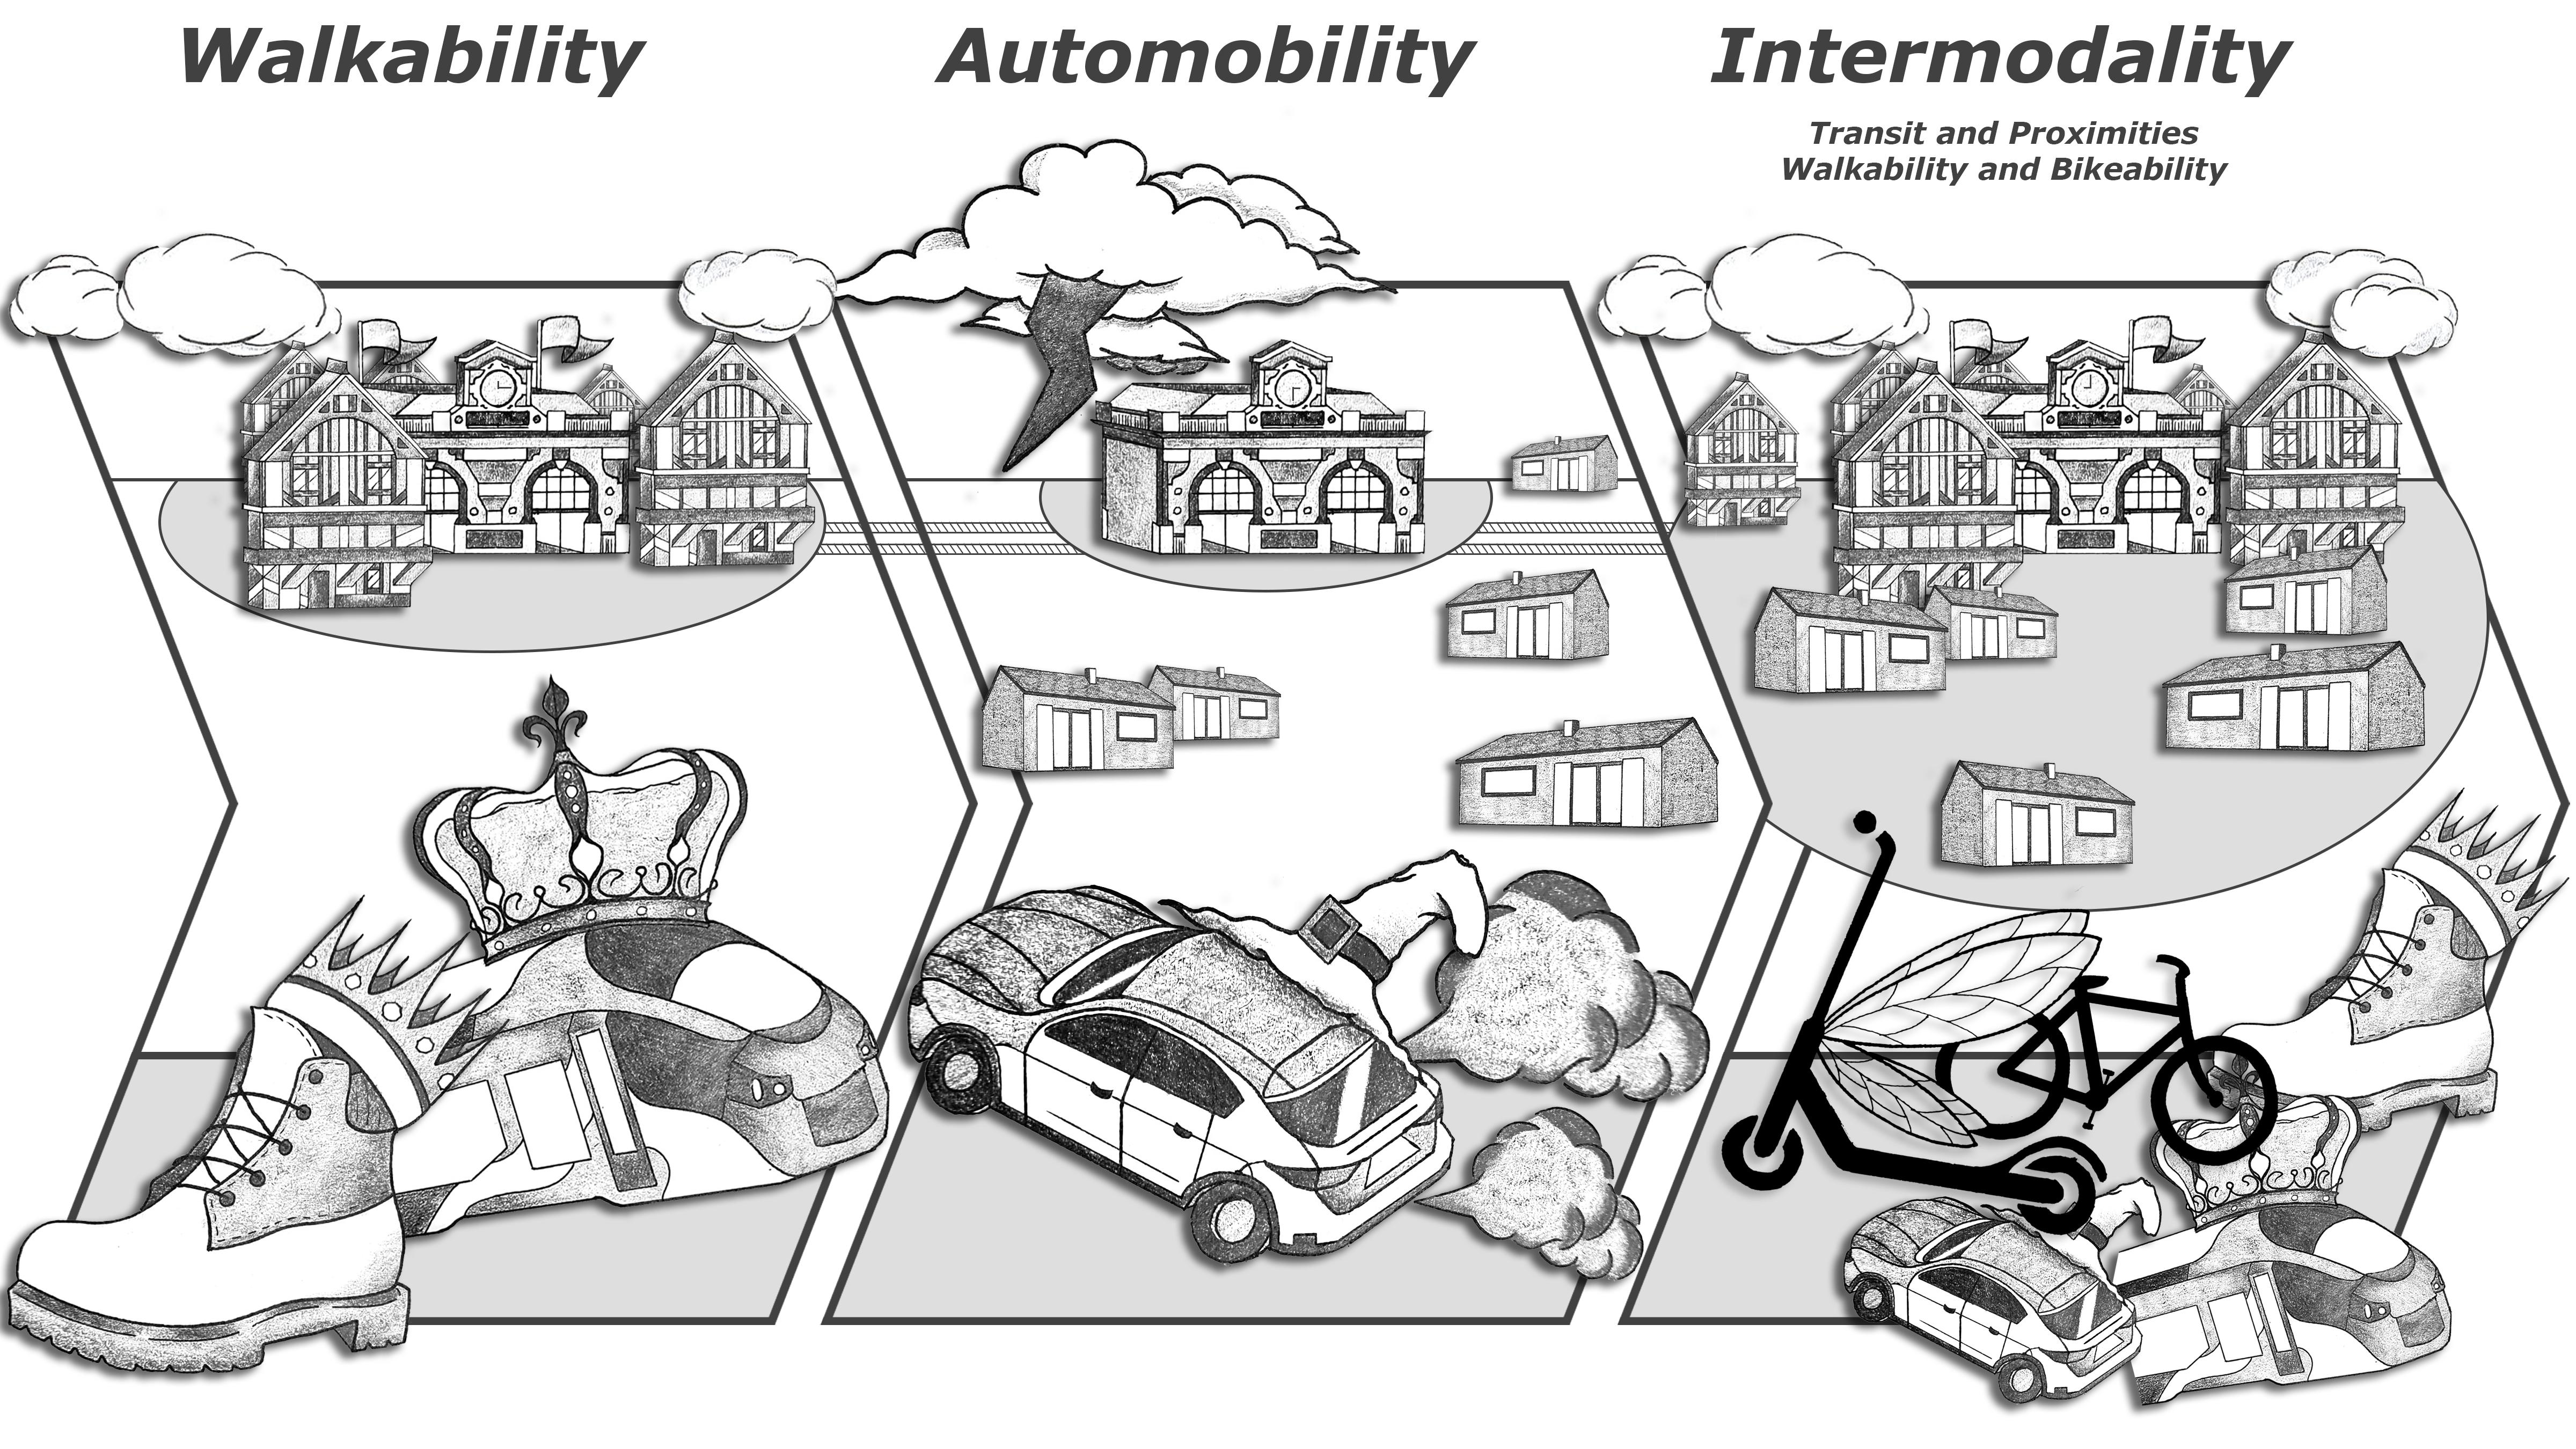
\includegraphics[width=1\columnwidth]{src/Figures/Preambule/EN_MT180_Illustration.jpg}}
        \vspace{5pt}
        \begin{flushright}\scriptsize{
        Author: \textcolor{blue}{Dylan Moinse (2022)}
        }\end{flushright}
    \end{figure}